\chapter{Planificación}

En este capítulo se presenta la planificación del desarrollo del proyecto \textit{NeuroForge}, definiendo la metodología iterativa empleada, la organización temporal del trabajo, los recursos y herramientas utilizados, las restricciones existentes y los riesgos identificados. Asimismo, se detallan las variaciones y desviaciones sufridas respecto al cronograma inicial y se incluye un estudio económico exhaustivo para evaluar los costes y la viabilidad comercial del videojuego tanto en un escenario individual como empresarial.

La planificación se ha concebido como una guía flexible, susceptible de ser ajustada a lo largo del desarrollo conforme se adquiría una visión más precisa del alcance real del proyecto y de las dificultades técnicas asociadas a su implementación. 

% ─────────────────────────────────────────────────────────────────────────────
\section{Metodología empleada}
% ─────────────────────────────────────────────────────────────────────────────

El desarrollo del TFG se ha llevado a cabo siguiendo una adaptación del \textit{Proceso Unificado}~\cite{cabalar_metodologias} (\textit{Unified Process}, UP), un marco de desarrollo de software caracterizado por estar dirigido por casos de uso, centrado en la arquitectura y, sobre todo, por ser \textit{iterativo e incremental}~\cite{solano2020}.

La distinción entre los términos \textit{iterativo} e \textit{incremental} es relevante. El componente \textit{iterativo} hace referencia a la repetición sistemática de un conjunto de disciplinas en cada ciclo de trabajo. El componente \textit{incremental} implica que el resultado de cada iteración es un incremento funcional que se integra con el trabajo anterior y contribuye directamente al producto final. En la Figura~\ref{fig:Metodologia} se presenta una metáfora visual que ilustra el carácter iterativo e incremental del proceso, en la que cada ciclo produce un incremento funcional que se integra con el trabajo anterior.

Para este proyecto, el Proceso Unificado organiza el ciclo de vida en cuatro grandes fases:

\begin{itemize}
	\item \textbf{Inicio:} Se establece el alcance del sistema, se identifican los casos de uso principales y se evalúa la viabilidad.
	\item \textbf{Elaboración:} Se refina la arquitectura del sistema, se detallan los requisitos más relevantes y se mitigan los riesgos técnicos críticos.
	\item \textbf{Construcción:} Constituye el núcleo del desarrollo, donde el sistema se construye de forma iterativa e incremental.
	\item \textbf{Transición:} El sistema se despliega, se realizan pruebas de integración definitivas y se produce la versión de entrega.
\end{itemize}

\begin{figure}[h!]
	\centering
	\includegraphics[width=0.8\linewidth]{../Imagenes/Metodologia}
	\caption{Metáfora gráfica del desarrollo iterativo e incremental}
	\label{fig:Metodologia}
\end{figure}

\subsection{Etapas de desarrollo y ordenación en la planificación}

Para cumplir con el rigor metodológico en un ámbito de desarrollo individual, el proyecto se ha estructurado en etapas secuenciales y disciplinas transversales que dictan el orden estricto de la planificación temporal. Estas etapas se ejecutan de la siguiente manera:

\begin{enumerate}
	\item \textbf{Etapa de Análisis Global y Requisitos:} Configura el punto de partida del proyecto (Fase de Inicio). Su objetivo es la definición formal de los requisitos funcionales y no funcionales del sistema, modelando los actores y el alcance técnico indispensable antes de escribir código.
	\item \textbf{Etapa de Diseño de Arquitectura Base:} Establece las bases estructurales del software (Fase de Elaboración). En ella se define la jerarquía de escenas en Godot, el modelo de datos del tablero y la abstracción de las piezas.
	\item \textbf{Etapas de Construcción Iterativa e Incremental:} Una vez fijados el análisis y el diseño globales, el trabajo se ordena en bloques funcionales que ejecutan internamente las disciplinas de desarrollo de manera cíclica:
	\begin{itemize}
		\item \textit{Implementación:} Codificación concreta en el motor Godot utilizando C\#.
		\item \textit{Pruebas unitarias y de caja negra:} Verificación inmediata de que cada nuevo incremento funcional responde a lo esperado sin romper los sistemas previos.
	\end{itemize}
	\item \textbf{Etapa de Transición y Pulido:} Bloque final orientado a la consolidación del sistema, optimización de rendimiento y pruebas de integración globales.
\end{enumerate}

Esta estructura metodológica se traslada directamente a la línea temporal del proyecto, ordenando las tareas cronológicamente desde la concepción teórica (Análisis y Diseño) hasta la materialización técnica y su posterior pulido en cinco iteraciones sucesivas. La correspondencia exacta se detalla en la Tabla~\ref{tab:fases_up}.

\begin{table}[H]
	\centering
	\begin{tabular}{|c|p{0.32\textwidth}|p{0.45\textwidth}|}
		\hline
		\textbf{Etapa} & \textbf{Iteración} & \textbf{Objetivo principal} \\
		\hline
		Inicio & Análisis & Visión, requisitos y alcance formal del sistema \\
		\hline
		Elaboración & Diseño & Arquitectura base, esquema de datos y escenas \\
		\hline
		& It. 1: Videojuego base & Núcleo jugable mínimo y lógicas de tablero \\ \cline{2-3}
		& It. 2: Interfaz de usuario & Interfaz, menús y flujo de navegación visual \\ \cline{2-3}
		& It. 3: Mejoras audiovisuales & Sonido, música y ambientación del entorno \\ \cline{2-3}
		\multirow{-4}{*}{Construcción} & It. 4: Bot inteligente & Implementación y entrenamiento de la IA \\
		\hline
		Transición & It. 5: Pulido final & Optimización, corrección de errores y entrega \\
		\hline
	\end{tabular}
	\caption{Correspondencia entre las fases de la metodología y la ordenación de las tareas en la planificación}
	\label{tab:fases_up}
\end{table}

% ─────────────────────────────────────────────────────────────────────────────
\section{Planificación inicial}
% ─────────────────────────────────────────────────────────────────────────────

La planificación inicial del proyecto se realizó con el objetivo de establecer una estimación razonable del trabajo a desarrollar, sirviendo como referencia para organizar las tareas y distribuir el esfuerzo a lo largo del periodo de realización del TFG. 

A petición metodológica, el análisis y el diseño conceptual se han extraído y unificado como tareas de entidad propia al inicio del cronograma para garantizar una base teórica sólida. El resto del desarrollo se distribuye en cinco iteraciones incrementales bien acotadas, manteniendo intacto el presupuesto temporal total de 300 horas.

% ─────────────────────────────────────────────────────────────────────────────
\subsection{Tareas Globales Iniciales: Análisis y Diseño}
% ─────────────────────────────────────────────────────────────────────────────

Estas dos tareas constituyen el cimiento del proyecto antes de proceder a cualquier tipo de implementación en el motor de videojuegos.

\begin{itemize}
	\item \textbf{Análisis de requisitos y casos de uso (6 h):} Identificación detallada de los requisitos funcionales del videojuego, definición de los actores (jugador, bot) y especificación formal de los casos de uso principales (despliegue de piezas, movimiento, combate y condiciones de victoria).
	\item \textbf{Diseño de la arquitectura y el modelo de datos (8 h):} Definición de la estructura de escenas madre en Godot, el esquema de clases principal en C\#, la representación interna del tablero matricial, las piezas y el modelado conceptual del sistema de toma de decisiones del bot.
\end{itemize}

% ─────────────────────────────────────────────────────────────────────────────
\subsection{Iteración 1: Núcleo jugable (Videojuego base)}
% ─────────────────────────────────────────────────────────────────────────────

El objetivo de esta iteración es desarrollar un \textit{Producto Mínimo Viable} funcional ---sin elementos visuales pulidos ni inteligencia artificial compleja--- que sirva como base estructural para el resto del proyecto y permita validar las decisiones técnicas adoptadas. Se estima una dedicación de \textbf{17~horas}.

\begin{itemize}
	\item \textbf{Tablero y casillas} (2~h): Implementación de la cuadrícula de $10\times10$ casillas, incluyendo las zonas intransitables del centro del tablero.
	\item \textbf{Definición de piezas} (3~h): Desarrollo de los distintos tipos de piezas con sus propiedades individuales: rangos, piezas inmóviles, y reglas especiales de combate y movimiento.
	\item \textbf{Sistema de movimiento} (3~h): Implementación de la selección de piezas, la visualización de las casillas de destino válidas y el desplazamiento sobre una casilla válida.
	\item \textbf{Sistema de combate} (3~h): Resolución inmediata de los enfrentamientos entre piezas según las reglas de rango definidas, sin animaciones ni retroalimentación visual elaborada.
	\item \textbf{Sistema de ocultación de piezas} (2~h): Implementación de la mecánica de identidades ocultas, de forma que las piezas rivales no muestran su tipo hasta que entran en combate.
	\item \textbf{Despliegue inicial aleatorio del bot} (1~h): Colocación automática de las piezas del oponente en su zona de despliegue de forma aleatoria al comienzo de la partida.
	\item \textbf{Bot de movimiento aleatorio} (1~h): Implementación de un oponente básico que ejecuta movimientos válidos de forma aleatoria durante su turno, actuando como versión mínima funcional del oponente.
	\item \textbf{Sistema de despliegue del jugador} (1~h): Pantalla básica que permite al jugador colocar sus piezas en su zona antes de comenzar la partida.
	\item \textbf{Condición de fin de partida} (1~h): Detección de las condiciones de victoria y derrota, con parada completa de la partida al producirse alguna de ellas.
\end{itemize}

\subsection{Iteración 2: Interfaz de usuario}
% ─────────────────────────────────────────────────────────────────────────────

El objetivo de esta iteración es dotar al videojuego de una interfaz completa, visualmente cuidada e intuitiva. Para dar cabida al bloque de Diseño global inicial, esta iteración reajusta su peso a \textbf{50 horas} sin perder alcance, optimizando las tareas de bocetado e integración.

\begin{itemize}
	\item \textbf{Bocetado de interfaces} (6~h): Elaboración de bocetos y propuestas visuales para todas las pantallas del videojuego antes de su implementación.
	\item \textbf{Búsqueda e integración de assets} (6~h): Selección de recursos gráficos para construir las interfaces de forma visualmente coherente.
	\item \textbf{Animaciones de movimiento de piezas} (1~h): Incorporación de animaciones básicas al desplazamiento de las piezas sobre el tablero.
	\item \textbf{Rediseño visual del tablero} (4~h): Mejora de la representación gráfica del tablero y de los indicadores de selección.
	\item \textbf{Sprites de las piezas} (10~h): Creación e integración de la representación gráfica de cada tipo de pieza.
	\item \textbf{Interfaz de despliegue mejorada} (4~h): Rediseño de la pantalla de colocación inicial de piezas.
	\item \textbf{Interfaz de resolución de combate} (6~h): Pantalla que muestra el resultado de cada enfrentamiento de forma explícita.
	\item \textbf{Pantalla de fin de partida} (1~h): Escena que informa al jugador del resultado final de la partida.
	\item \textbf{Menú principal} (1~h): Escena inicial con opciones para comenzar, consultar reglas y salir.
	\item \textbf{Menú de pausa} (2~h): Escena accesible durante la partida.
	\item \textbf{Menú de reglas} (6~h): Escena explicativa de las mecánicas y reglas del juego.
	\item \textbf{Ajustes y correcciones} (3~h): Revisión general de los elementos implementados.
\end{itemize}

\subsection{Iteración 3: Mejoras audiovisuales}
% ─────────────────────────────────────────────────────────────────────────────

El objetivo de esta iteración es completar la experiencia audiovisual del videojuego mediante la incorporación de sonido y los últimos elementos visuales de ambientación. Se estima una dedicación de \textbf{15 horas}.

\begin{itemize}
	\item \textbf{Fondos y elementos decorativos} (2~h): Incorporación de fondos y elementos visuales de carácter estético.
	\item \textbf{Efectos de sonido} (6~h): Integración de efectos sonoros asociados a las distintas acciones del videojuego.
	\item \textbf{Música} (3~h): Incorporación de música de fondo para las distintas escenas del videojuego.
	\item \textbf{Menú de opciones de audio} (4~h): Implementación de una pantalla de configuración para ajustar volúmenes.
\end{itemize}

\subsection{Iteración 4: Implementación del bot inteligente}
% ─────────────────────────────────────────────────────────────────────────────

El objetivo de esta iteración es desarrollar el sistema de inteligencia artificial estratégico. Puesto que el diseño conceptual de la IA se ha absorbido en la tarea de Diseño global inicial, esta iteración pasa a centrarse puramente en su desarrollo técnico, entrenamiento y validación, reduciendo su cómputo a \textbf{40 horas}.

\begin{itemize}
	\item \textbf{Desarrollo de la lógica algorítmica del modelo} (18~h): Programación del motor de toma de decisiones e integración de las matrices de pesos para gestionar la información oculta del rival.
	\item \textbf{Entrenamiento del modelo} (10~h): Proceso de optimización de la IA mediante partidas simuladas contra versiones previas de sí misma.
	\item \textbf{Integración del bot inteligente} (5~h): Sustitución del bot aleatorio y acoplamiento directo con el sistema de turnos de la arquitectura.
	\item \textbf{Evaluación y balanceo del comportamiento} (7~h): Pruebas intensivas del bot frente a jugadores humanos y escenarios límite para garantizar decisiones coherentes y sin bloqueos.
\end{itemize}

\subsection{Iteración 5: Pulido final}
% ─────────────────────────────────────────────────────────────────────────────

El objetivo de esta última iteración es revisar el conjunto del sistema, corregir los errores detectados y garantizar la estabilidad y calidad del producto. Se estima una dedicación de \textbf{14 horas}.

\begin{itemize}
	\item \textbf{Optimización del rendimiento} (4~h): Análisis y mejora del rendimiento del sistema, hilos de ejecución y consumos de recursos.
	\item \textbf{Revisión del feedback al jugador} (4~h): Comprobación de que toda la información visual y sonora se transmite de forma limpia.
	\item \textbf{Corrección de errores} (4~h): Detección y resolución de bugs.
	\item \textbf{Pruebas de integración} (2~h): Verificación final del build completo del videojuego.
\end{itemize}

Paralelamente al desarrollo técnico, se estiman exactamente \textbf{140 horas} para la elaboración progresiva de la memoria del TFG, incluyendo la descripción del diseño del videojuego, la justificación de las decisiones técnicas adoptadas y el análisis de los resultados obtenidos.

En conjunto, la estimación total de dedicación para el proyecto asciende a unas \textbf{300 horas}, distribuidas de forma exacta en, 14 horas de tareas globales (Análisis y Diseño), 136 horas de desarrollo técnico y pulido en las cinco iteraciones, y las 140 restantes a la documentación de la memoria.

La Tabla~\ref{tab:iteraciones} recoge el resumen definitivo de los tiempos de desarrollo adaptados.

\begin{table}[H]
	\centering
	\begin{tabular}{|c|p{0.48\textwidth}|c|c|}
		\hline
		\textbf{Etapa / It.} & \textbf{Descripción de la Tarea} & \textbf{Horas est.} & \textbf{Fecha est. fin.} \\
		\hline
		Tarea Global & Análisis de requisitos y casos de uso & 6 h & 2026-02-05 \\
		\hline
		Tarea Global & Diseño de arquitectura y datos & 8 h & 2026-02-12 \\
		\hline
		1 & Implementación del videojuego base & 17 h & 2026-02-26 \\
		\hline
		2 & Interfaz de usuario y pulido visual & 50 h & 2026-04-05 \\
		\hline
		3 & Mejoras audiovisuales & 15 h & 2026-04-19 \\
		\hline
		4 & Implementación del bot inteligente (IA) & 40 h & 2026-05-31 \\
		\hline
		5 & Pulido final e integración & 14 h & 2026-06-07 \\
		\hline
		- & Documentación de la Memoria (Paralela) & 140 h & 2026-06-14 \\
		\hline
		\multicolumn{2}{|p{0.56\textwidth}|}{\textbf{Total}} & \textbf{300 h} & \\
		\hline
	\end{tabular}
	\caption{Distribución ajustada de horas por tareas globales e iteraciones del proyecto}
	\label{tab:iteraciones}
\end{table}

La Figura \ref{fig:gantt1} y \ref{fig:gantt2} muestra de manera de manera actualizada el cronograma con la inserción de las tareas macro de análisis y diseño al inicio del desarrollo.

\begin{landscape}
	\begin{figure}[H]
		\centering
		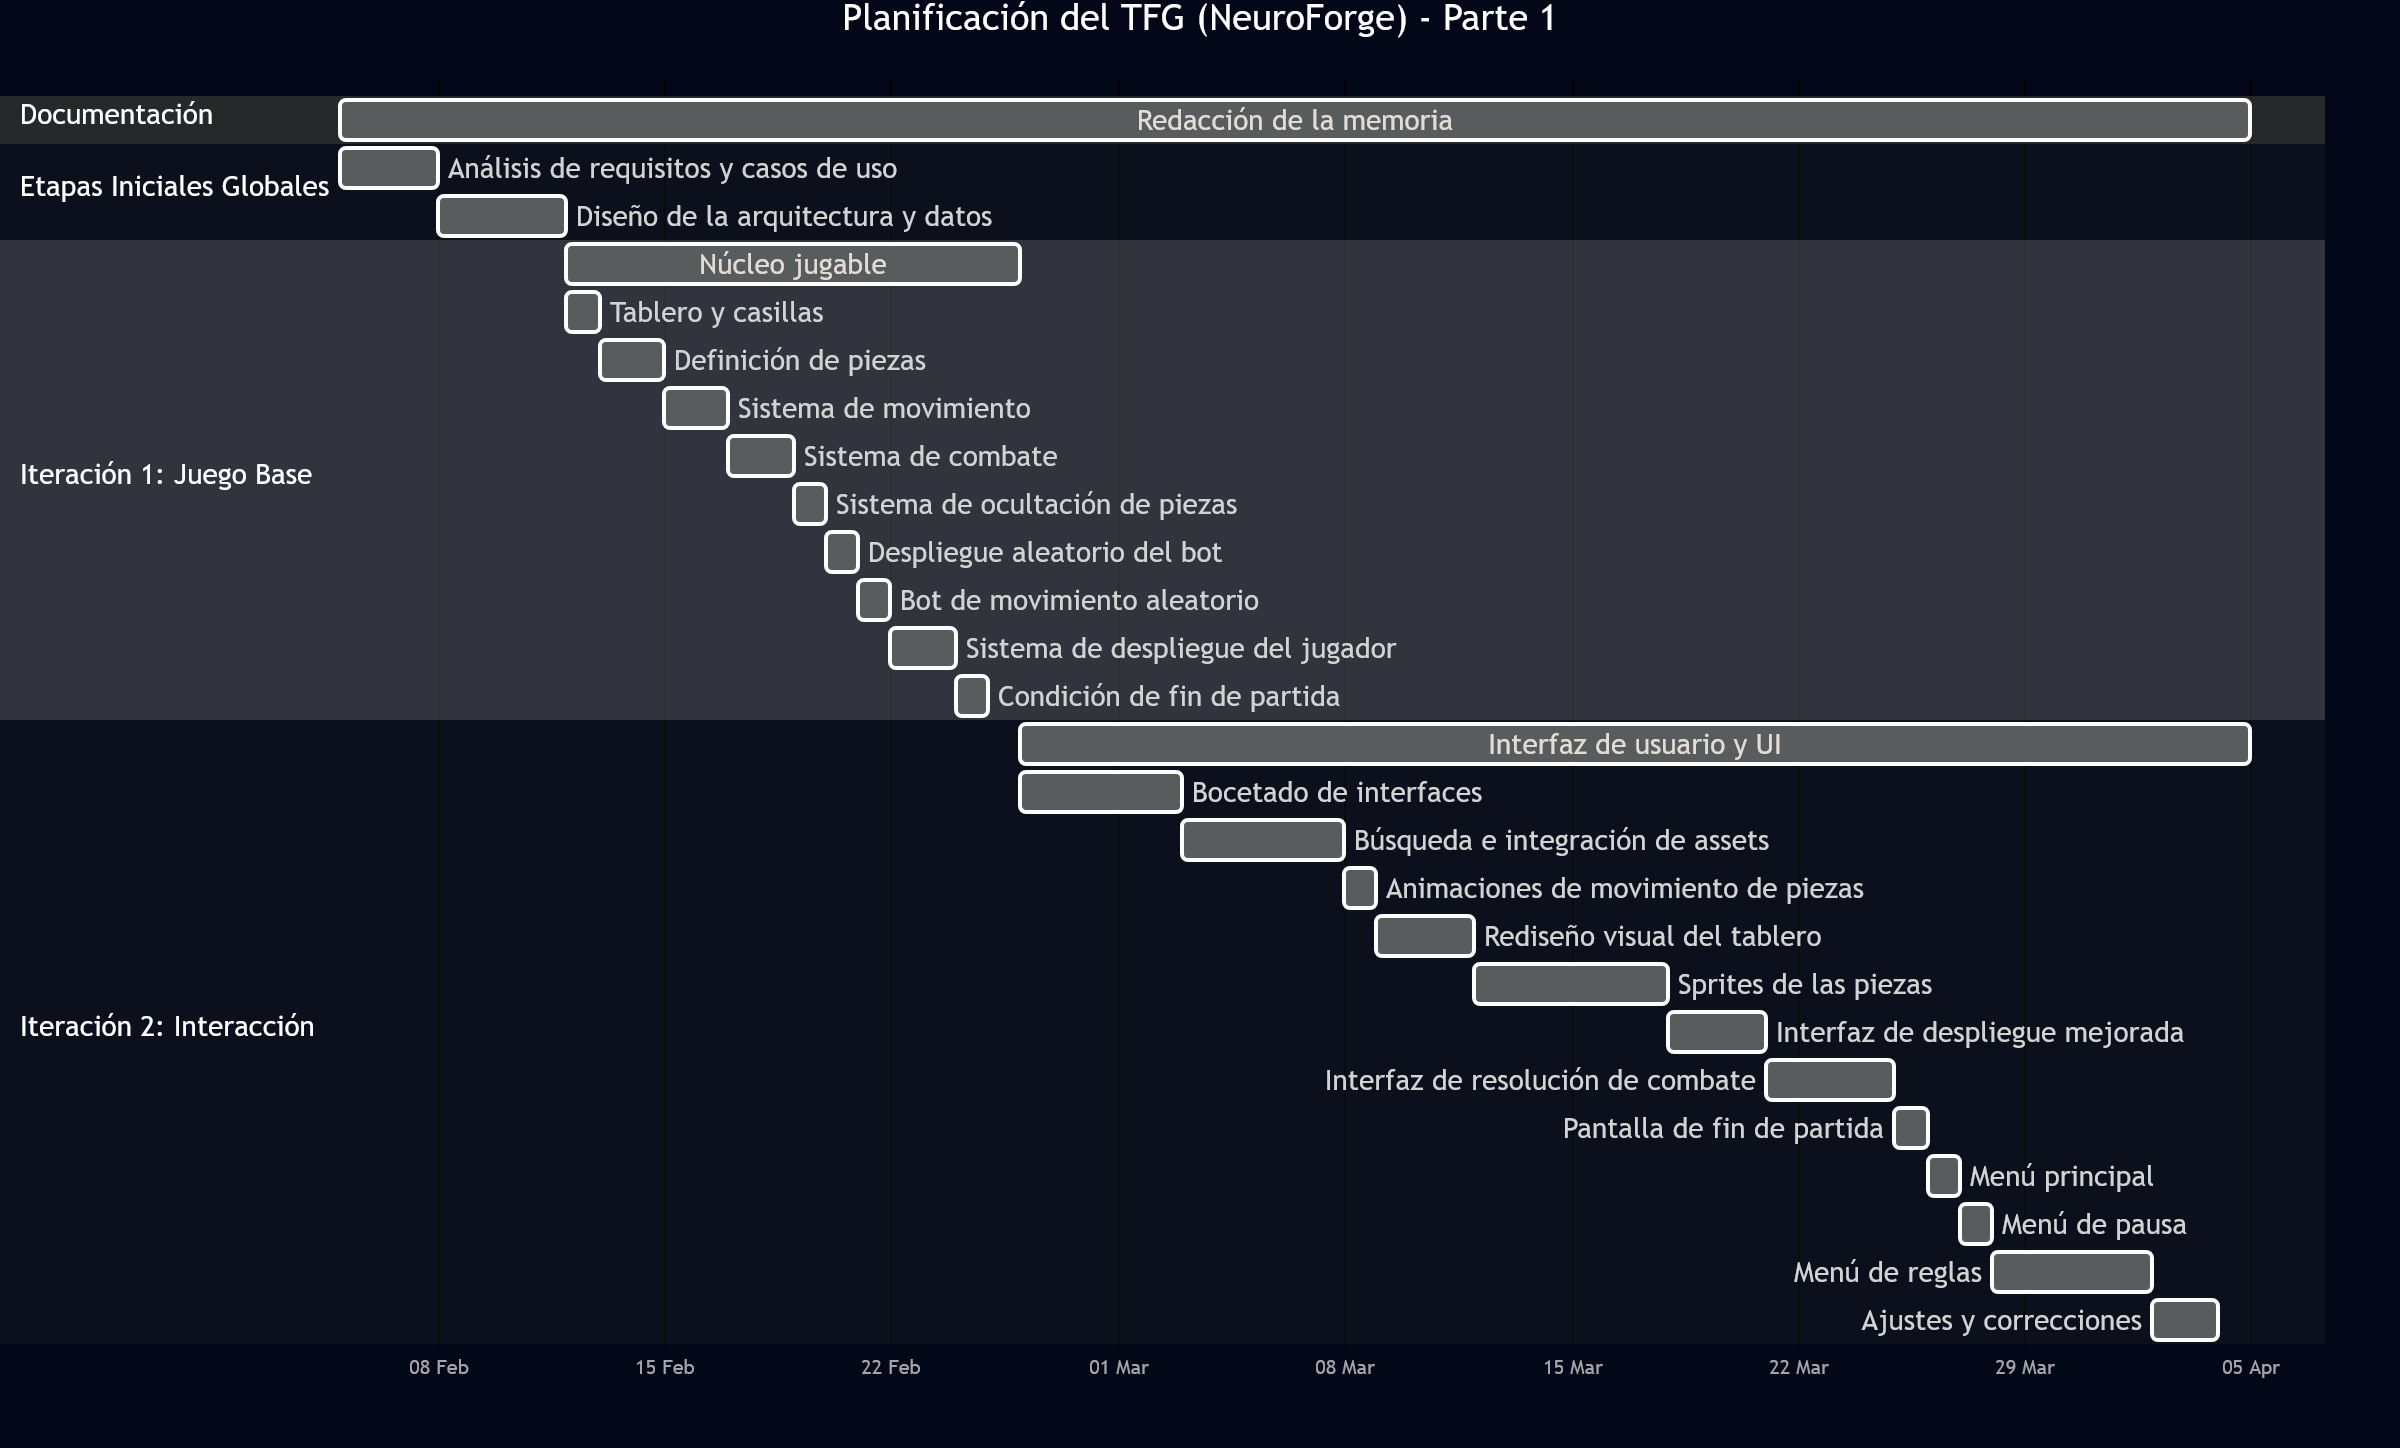
\includegraphics[width=\linewidth]{../Imagenes/Gantt1.png} 
		\caption{Parte 1 del diagrama de Gantt general del desarrollo del TFG}
		\label{fig:gantt1}
	\end{figure}
	\begin{figure}[H]
		\centering
		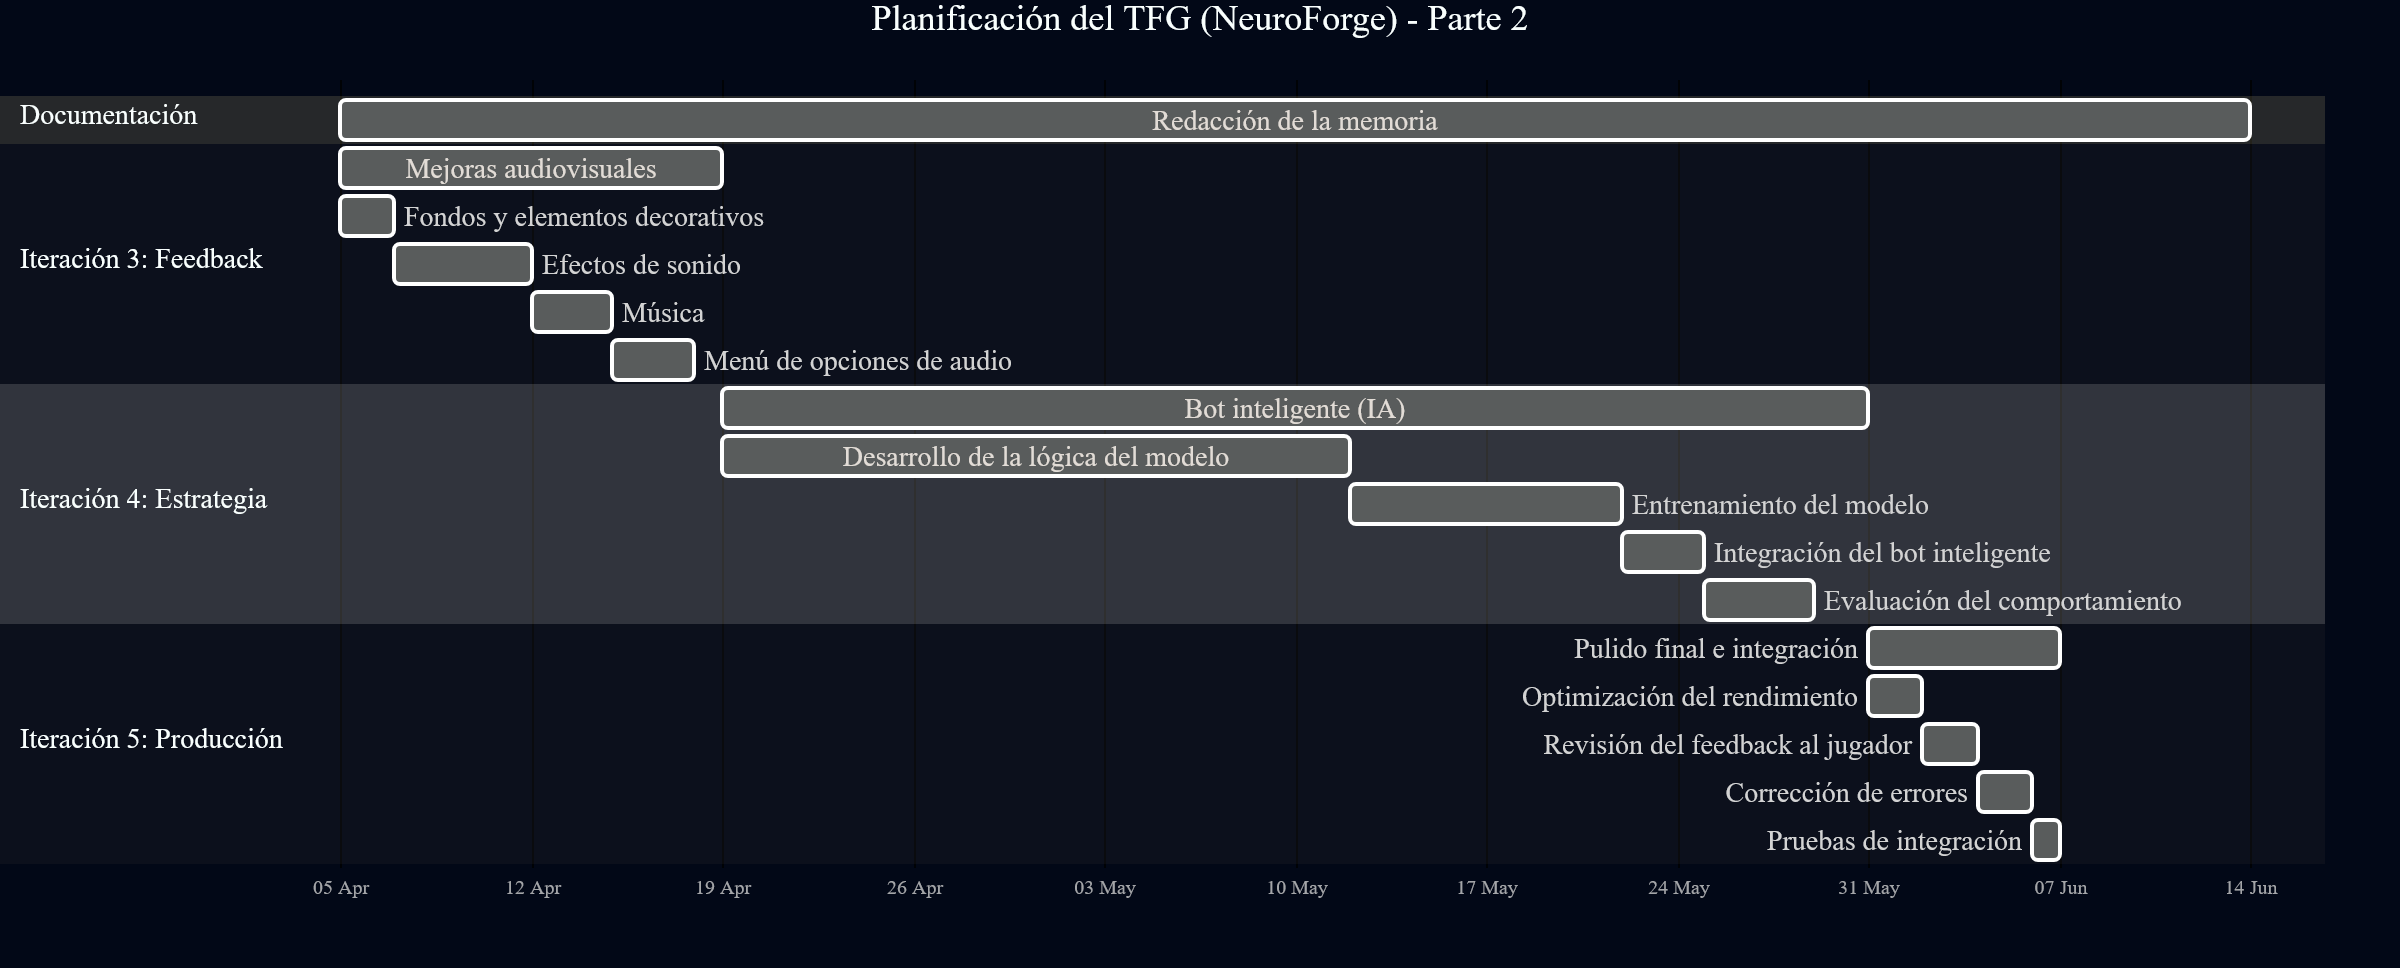
\includegraphics[width=\linewidth]{../Imagenes/Gantt2} 
		\caption{Parte 2 del diagrama de Gantt general del desarrollo del TFG}
		\label{fig:gantt2}
	\end{figure}
 \end{landscape}
 
% ─────────────────────────────────────────────────────────────────────────────
\section{Riesgos}
% ─────────────────────────────────────────────────────────────────────────────

Durante la fase de planificación se identificaron distintos riesgos que podrían afectar al correcto desarrollo del proyecto, recogidos en la Tabla~\ref{tab:riesgos}. Para cada uno se ha analizado su naturaleza e impacto potencial, definiendo medidas de contingencia orientadas a minimizar sus efectos en caso de materializarse.

La identificación temprana de estos riesgos permite anticipar posibles problemas técnicos y organizativos, facilitando la toma de decisiones durante el desarrollo y contribuyendo a mantener la estabilidad del proyecto.

\begin{table}[H]
	\centering
	\begin{tabular}{|
			>{\centering\arraybackslash}p{4cm}|
			>{\centering\arraybackslash}p{2.5cm}|
			>{\centering\arraybackslash}p{2cm}|
			>{\centering\arraybackslash}p{6cm}|}
		\hline
		\textbf{Riesgo} & \textbf{Tipo} & \textbf{Impacto} &
		\textbf{Plan de contingencia} \\
		\hline
		\textbf{R1:} Fallos del motor o incompatibilidades
		& Técnico & Alto
		& Revisar dependencias y adaptar los scripts afectados. \\
		\hline
		\textbf{R2:} Retrasos en el cronograma
		& Temporal & Medio
		& Reajustar tareas no prioritarias y reducir funcionalidades accesorias. \\
		\hline
		\textbf{R3:} Errores en el bot o en las reglas del videojuego
		& Técnico & Medio
		& Simplificar el comportamiento de la IA y priorizar la estabilidad de las mecánicas fundamentales. \\
		\hline
		\textbf{R4:} Pérdida de datos o código fuente
		& Técnico & Alto
		& Uso de control de versiones y copias de seguridad en la nube. \\
		\hline
		\textbf{R5:} Falta de tiempo para pruebas y ajuste del videojuego
		& Temporal & Alto
		& Priorizar pruebas de jugabilidad y corregir únicamente los errores críticos. \\
		\hline
		\textbf{R6:} Carencia de recursos gráficos o sonoros adecuados
		& Logístico & Bajo
		& Crear recursos propios o adaptar recursos de terceros de libre uso. \\
		\hline
		\textbf{R7:} Incapacidad temporal para el desarrollo
		& Temporal & Alto
		& Reorganizar tareas, priorizar funcionalidades críticas y ajustar el cronograma. \\
		\hline
		\textbf{R8:} Dificultad en el diseño o implementación del bot inteligente
		& Técnico & Alto
		& Simplificar el modelo de decisión si fuera necesario; mantener operativo el bot aleatorio como versión mínima funcional. \\
		\hline
		\textbf{R9:} Bloqueos por depuración de errores difíciles
		& Técnico & Medio
		& Mantener control de versiones; realizar pruebas frecuentes; documentar los problemas encontrados y consultar la documentación oficial de Godot y C\#. \\
		\hline
	\end{tabular}
	\caption{Riesgos identificados y planes de contingencia}
	\label{tab:riesgos}
\end{table}

% ─────────────────────────────────────────────────────────────────────────────
\section{Restricciones}
% ─────────────────────────────────────────────────────────────────────────────

El desarrollo de \textit{NeuroForge} ha estado condicionado por una serie
de restricciones que han influido directamente en la planificación, la
selección de herramientas y el alcance final del proyecto.

\begin{itemize}
	
	\item \textbf{Técnicas:} Se establece el uso del motor \textit{Godot} junto con el lenguaje de programación \textit{C\#}. Aunque Godot emplea de forma nativa GDScript, se ha optado por C\# debido a su soporte oficial y su mayor adecuación al perfil del proyecto. Asimismo, se limita el uso a librerías y recursos gratuitos o de código abierto.
	
	\item \textbf{Temporales:} El desarrollo se limita al periodo de realización del TFG, lo que impone una duración finita y condiciona directamente el número de funcionalidades que pueden implementarse.
	
	\item \textbf{Económicas:} No se dispone de presupuesto para la adquisición de licencias de software de pago, la contratación de colaboradores ni la compra de recursos gráficos o sonoros.
	
	\item \textbf{Personales:} El proyecto es desarrollado íntegramente por un único estudiante, lo que limita la paralelización de tareas y exige una gestión eficiente del tiempo disponible.
	
	\item \textbf{Académicas:} El trabajo debe ajustarse a la normativa, estructura y requisitos establecidos por la Escuela de Ingeniería Informática de Valladolid para los Trabajos de Fin de Grado.
	
\end{itemize}

% ─────────────────────────────────────────────────────────────────────────────
\section{Herramientas}
% ─────────────────────────────────────────────────────────────────────────────

Para llevar a cabo este Trabajo Fin de Grado, ha sido necesario seleccionar un conjunto integrado de herramientas de software que abarquen todas las necesidades del ciclo de vida del proyecto, desde la propia implementación del videojuego hasta la gestión de tareas, el diseño de recursos y la redacción de esta memoria. 

A continuación, se detalla en primer lugar el análisis y la elección de la pieza central del entorno de desarrollo, el motor de videojuegos, para posteriormente describir el resto de herramientas complementarias que conforman el flujo de trabajo.

\clearpage

\subsection{Selección del Motor de Videojuegos}

Un motor de videojuegos es un \textit{framework} de desarrollo que proporciona un conjunto integrado de herramientas, librerías y sistemas sobre los que construir un videojuego, abstrayendo tareas como el renderizado gráfico, la gestión de escenas, el control de entrada del usuario, la simulación de físicas o la exportación a distintas plataformas.

Tal como se describe en el capítulo de Antecedentes, el panorama actual del desarrollo independiente está dominado por \textit{Unreal Engine}, \textit{Unity} y \textit{Godot}, tres motores con enfoques técnicos y modelos de licencia distintos. Para este proyecto se ha seleccionado \textbf{Godot} como motor de desarrollo por las siguientes razones técnicas:

\begin{itemize}
	\item Su motor 2D es un sistema nativo e independiente del motor 3D, lo que lo hace especialmente eficiente para un videojuego de estrategia por turnos bidimensional como \textit{NeuroForge}.
	\item Su editor ocupa menos de 200~MB y permite ciclos de iteración muy rápidos, ventaja significativa en un proyecto de desarrollo individual con restricciones temporales.
	\item Se distribuye bajo licencia MIT, eliminando cualquier coste de licencia y garantizando que las condiciones de uso no pueden cambiar de forma unilateral~\cite{godot_features}.
	\item La escala del proyecto no requiere el ecosistema de extensiones de los motores comerciales, por lo que la comunidad más reducida de Godot no supone ninguna restricción práctica.
\end{itemize}

El desarrollo se ha realizado concretamente sobre \textit{Godot} en su versión~4.6.1. Su editor visual se ha utilizado para la composición y gestión de escenas, la definición de nodos y señales, la configuración de la interfaz de usuario mediante el sistema de nodos \textit{Control}, y la gestión de recursos gráficos y sonoros. Su sistema de exportación ha permitido generar ejecutables de escritorio sin dependencias externas, facilitando la distribución del producto final.

\subsection{Otras herramientas utilizadas}

Una vez determinada la elección de Godot como núcleo tecnológico, se seleccionó un conjunto de herramientas de soporte atendiendo a criterios de adecuación técnica, disponibilidad gratuita o bajo coste, compatibilidad con el motor y facilidad de integración en el flujo de trabajo del proyecto. 

El desarrollo del videojuego se ha realizado concretamente sobre el motor \textit{Godot} en su versión 4.6.1. Godot ha servido como entorno integral de desarrollo, su editor visual se ha utilizado para la composición y gestión de escenas, la definición de nodos y señales, la configuración de la interfaz de usuario mediante el sistema de nodos \textit{Control}, y la gestión de recursos gráficos y sonoros. Además, su sistema de exportación ha permitido generar ejecutables de escritorio sin dependencias externas, facilitando la distribución del producto final.

\clearpage

Como lenguaje de programación se ha empleado \textit{C\#} sobre el entorno de ejecución .NET~9.0, que cuenta con soporte oficial dentro de la versión de Godot utilizada. La elección de \textit{C\#} frente a \textit{GDScript}, el lenguaje nativo del motor, se debe a varias razones. Su sistema de tipado estático y fuerte reduce los errores en tiempo de compilación, su orientación a objetos facilita la organización de un proyecto con múltiples sistemas interrelacionados (tablero, piezas, combate, IA), y su amplia adopción en la industria del desarrollo de software proporciona una base de conocimiento y herramientas de depuración más maduras.

El control de versiones del proyecto se ha gestionado mediante \textit{Git}, utilizando \textit{GitHub} como plataforma de alojamiento del repositorio remoto. Git ha permitido mantener un historial completo de todos los cambios realizados en el código fuente, revertir modificaciones problemáticas y trabajar en ramas experimentales sin riesgo para la línea principal de desarrollo. GitHub, por su parte, ha proporcionado una copia de seguridad permanente en la nube y ha facilitado la revisión del código mediante su interfaz web. Se ha utilizado un flujo de trabajo basado en \textit{commits} frecuentes, organizados por funcionalidad o tarea completada.

Para la creación y edición de los recursos gráficos del videojuego se han empleado \textit{Aseprite}. \textit{Aseprite} es un editor especializado en \textit{pixel art}, utilizado para diseñar los sprites de las piezas, los elementos de la interfaz y modificar los assets de terceros. Su soporte nativo para capas, paletas de color y hojas de sprites (\textit{sprite sheets}) lo convierte en una herramienta especialmente adecuada para el estilo visual del proyecto. Paint se ha utilizado de forma complementaria para ediciones rápidas y ajustes menores sobre recursos ya existentes.

La gestión del apartado sonoro se ha apoyado en \textit{Audacity}, un editor de audio de código abierto que ha permitido recortar, normalizar y ajustar el volumen de los efectos de sonido antes de integrarlos en el motor. Los recursos de audio se han obtenido de las plataformas \textit{Freesound} y \textit{Pixabay}, ambas repositorios de efectos sonoros y pistas musicales de libre uso bajo licencias compatibles con proyectos de esta naturaleza. La combinación de estas herramientas ha permitido dotar al videojuego de un apartado sonoro coherente sin necesidad de recurrir a recursos de pago.

La redacción y maquetación de la presente memoria se ha realizado íntegramente mediante \textit{\LaTeX}, un sistema de composición tipográfica ampliamente utilizado en el ámbito académico y científico. \LaTeX{} ha facilitado la gestión de la estructura del documento, la numeración automática de secciones, figuras y tablas, la generación de referencias cruzadas y la compilación de la bibliografía mediante Bib\LaTeX. Su capacidad para separar contenido y formato ha resultado especialmente útil durante las revisiones sucesivas del documento.

Finalmente, la planificación y el seguimiento del proyecto se han gestionado a través de \textit{Notion}, una herramienta de productividad y gestión de contenido. Notion ha servido como eje organizativo del proyecto, se ha utilizado para llevar a cabo las fases de desarrollo y sus hitos asociados, mantener un registro de las horas invertidas en cada tarea, anotar correcciones y decisiones de diseño pendientes, y elaborar borradores previos a su incorporación a la memoria. También se ha empleado \textit{Mermaid} como soporte para la construcción del diagrama de Gantt y para el seguimiento del progreso global del trabajo.

A modo de síntesis, la Tabla~\ref{tab:Herramientas} ofrece un resumen de conjunto de todas las herramientas mencionadas y su rol dentro de la ejecución de este trabajo.

\clearpage

\begin{table}[h!]
	\centering
	\begin{tabularx}{\textwidth}{|
			>{\centering\arraybackslash}X|
			>{\centering\arraybackslash}X|
			>{\centering\arraybackslash}p{8cm}|}
		\hline
		\textbf{Tipo} & \textbf{Herramienta} & \textbf{Uso principal} \\
		\hline
		Motor de videojuegos & Godot 4.6.1 & Desarrollo integral del videojuego: escenas, lógica, interfaz y exportación. \\
		\hline
		Lenguaje de programación & C\# (.NET 9.0) & Implementación de la lógica del videojuego, sistemas de IA y scripts de control. \\
		\hline
		Lenguaje de IA y Entrenamiento & Python 3.x & Creación del entorno de Gymnasium, entrenamiento y optimización del bot. \\
		\hline
		Control de versiones & Git / GitHub & Historial de cambios, gestión de ramas y copia de seguridad en la nube. \\
		\hline
		Diseño gráfico & Aseprite & Creación de sprites en \textit{pixel art}, animaciones y edición de recursos visuales. \\
		\hline
		Audio & Audacity / Freesound / Pixabay & Edición de efectos sonoros y obtención de música y SFX de libre uso. \\
		\hline
		Documentación & \LaTeX{} / Bib\LaTeX & Redacción, maquetación y gestión bibliográfica de la memoria del TFG. \\
		\hline
		Gestión y planificación & Notion / Mermaid & Organización de fases, registro de horas, seguimiento de hitos y borradores. \\
		\hline
		IA Generativa & Claude & Asistencia para el uso de Latex y sugerencias de uso de Godot con C\# \\
		\hline
	\end{tabularx}
	\caption{Herramientas empleadas en el desarrollo del proyecto}
	\label{tab:Herramientas}
\end{table}

% ─────────────────────────────────────────────────────────────────────────────
\section{Variación de planificación}
% ─────────────────────────────────────────────────────────────────────────────

A lo largo del desarrollo del proyecto se han producido algunas variaciones respecto a la planificación inicial, aunque sin llegar a afectar de forma significativa al calendario general ni al alcance final del trabajo.

El cambio más relevante respecto a la planificación original fue la reorganización del orden de las iteraciones. En la planificación inicial se contemplaban cuatro iteraciones, en las que el desarrollo del bot inteligente se situaba en segundo lugar, antes del diseño de la interfaz de usuario. Sin embargo, durante el desarrollo se optó por invertir este orden, abordando primero la interfaz y posponiendo el bot a la cuarta iteración.

Esta decisión responde a una priorización deliberada del producto final. Dado que el bot inteligente constituye un objetivo secundario del proyecto, se consideró más adecuado garantizar primero la existencia de un videojuego completo y funcional de principio a fin, con una experiencia de juego clara y pulida. De este modo, aunque el desarrollo del bot no llegara a completarse en el tiempo disponible, el proyecto contaría en todo caso con un resultado presentable y jugable, apoyado en el bot aleatorio ya implementado en la primera iteración como oponente mínimo funcional. Como consecuencia de esta reorganización, la planificación pasó de cuatro a cinco iteraciones, separando las mejoras audiovisuales en una iteración propia. Este ajuste no supuso un incremento en el tiempo total estimado, sino una redistribución del trabajo en fases más cohesionadas.

\clearpage

En cuanto a las desviaciones cronológicas y de esfuerzo registradas, las dos primeras iteraciones experimentaron retrasos en sus fechas de entrega respecto a lo estimado. La primera iteración, cuyo núcleo jugable estaba previsto para el 26 de febrero, no se completó hasta el 19 de marzo. El motivo principal fue la necesidad de revisar y rediseñar aspectos del modelo de datos que no habían sido contemplados con suficiente detalle durante la fase de diseño inicial. Al comenzar la implementación se detectaron inconsistencias en la representación interna de las piezas y su relación con el tablero que obligaron a replantear parte de la arquitectura antes de poder continuar con el desarrollo. Esta revisión supuso una desviación de $+12$ horas de trabajo sobre el presupuesto de la tarea y desplazó la fecha de entrega de la iteración.

Como consecuencia directa de ese retraso en el calendario, la segunda iteración, dedicada a la interfaz de usuario y el pulido visual, también vio afectada su fecha de cierre, postergándose del 5 de abril al 18 del mismo mes. Sin embargo, en este caso no surgieron dificultades técnicas adicionales significativas, por lo que las horas estimadas de desarrollo se respetaron rigurosamente y la desviación temporal fue puramente un retraso arrastrado desde la iteración anterior.

A partir de este punto, la carga horaria planificada se estabilizó e incluso se logró optimizar el tiempo invertido en las fases restantes, contrarrestando el balance de horas del proyecto. La tercera iteración pudo completarse en la fecha estimada requiriendo $8$ horas menos de lo previsto gracias a la solidez de la arquitectura base ya corregida. Del mismo modo, la quinta iteración se cerró reduciendo en $4$ horas su estimación inicial. Esta recuperación del tiempo de desarrollo, sumada a una redistribución eficiente de las horas dedicadas en paralelo a la redacción de la memoria, permitió absorber por completo el sobrecoste horario de la primera iteración, finalizando el proyecto dentro del cómputo global de horas presupuestado.

La Tabla~\ref{tab:variacion} recoge el resumen de las desviaciones producidas respecto a la planificación inicial, detallando las fechas planificadas frente a las reales junto al balance neto de horas de cada fase.

\begin{table}[H]
	\centering
	\begin{tabular}{|c|p{0.35\textwidth}|c|c|c|}
		\hline
		\textbf{It.} & \textbf{Descripción} & \textbf{Fecha est.} & \textbf{Fecha real} & \textbf{Desviación (h)} \\
		\hline
		T. Global & Análisis y requisitos & 2026-02-05 & 2026-02-05 & 0 h \\
		\hline
		T. Global & Diseño de arquitectura & 2026-02-12 & 2026-02-12 & 0 h \\
		\hline
		1 & Videojuego base & 2026-02-26 & 2026-03-19 & +12 h \\
		\hline
		2 & Interfaz de usuario & 2026-04-05 & 2026-04-18 & 0 h \\
		\hline
		3 & Mejoras audiovisuales & 2026-04-19 & 2026-04-19 & -8 h \\
		\hline
		4 & Bot inteligente (IA) & 2026-05-31 & 2026-05-31 & 0 h \\
		\hline
		5 & Pulido final & 2026-06-07 & 2026-06-07 & -4 h \\
		\hline
		\multicolumn{2}{|l|}{\textbf{Balance Total de Desviación}} & \multicolumn{2}{c|}{} & \textbf{0 h} \\
		\hline
	\end{tabular}
	\caption{Variaciones en fechas de finalización y desviación respecto a la planificación inicial}
	\label{tab:variacion}
\end{table}

\clearpage

% ─────────────────────────────────────────────────────────────────────────────
\section{Costes del proyecto}
% ─────────────────────────────────────────────────────────────────────────────

A lo largo del desarrollo de este Trabajo Fin de Grado el estudiante no ha incurrido en ningún gasto económico directo, todas las herramientas empleadas son de código abierto o gratuitas, y el espacio de trabajo ha sido el domicilio particular. No obstante, con el fin de evaluar la viabilidad del videojuego en un entorno profesional, se presenta a continuación una estimación de los costes en los que se habría incurrido de haberse desarrollado en ese contexto. Se distinguen dos escenarios, el \textit{escenario individual}, que refleja el coste directo para un profesional autónomo, y el \textit{escenario empresarial}, que incorpora las cargas adicionales que asumiría una empresa al contratarlo.

\subsection{Costes de personal}

El coste de personal es el factor dominante en cualquier proyecto de desarrollo de software. Para estimarlo se toma como referencia el salario mensual bruto de un desarrollador junior de videojuegos en España, situado en aproximadamente \textit{2.333~€ brutos/mes} (28.000~€ anuales según datos de Glassdoor~\cite{glassdoor_gamedeveloper}). Dado que la dedicación total del proyecto ha sido de \textit{300~horas} y que una jornada laboral estándar supone unas 160~horas mensuales, la duración equivalente es de \textit{1,875~meses}, lo que da un coste salarial bruto de \textit{4.125,00~€}. Este es el coste en el escenario individual, lo que percibiría el profesional por su trabajo.

En el escenario empresarial, la organización asume además las cotizaciones a la Seguridad Social a su cargo, que en España suponen aproximadamente un 32\,\% adicional sobre el salario bruto~\cite{seguridad_social_costes}, elevando el coste real de personal para la empresa a \textit{5.445,00~€}.

\subsection{Costes de software}

Los costes de software varían según el escenario. En el escenario individual, un profesional autónomo debería adquirir por su cuenta las herramientas necesarias: Aseprite por 16,79~€ (pago único), Astah Professional en su licencia individual por 17,98~€ y Notion Plus por 22,10~€ durante los dos meses de desarrollo técnico efectivo, sumando \textit{56,87~€}~\cite{astah_pricing, astah_pricing_team, notion_pricing}. En el escenario empresarial, las licencias escalan a tarifas orientadas a organizaciones, Astah Professional pasa a su modalidad de licencia flotante anual a 180~€/año (15~€/mes) y Notion al plan Business a 20~USD/mes por usuario (aproximadamente 18,40~€/mes), lo que eleva el total de software empresarial a \textit{87,59~€} durante ese mismo periodo. Godot, Git y Audacity no generan coste en ninguno de los dos escenarios al distribuirse bajo licencias de código abierto.

\clearpage

\subsection{Costes de infraestructura}

Los costes de infraestructura difieren de forma significativa entre ambos escenarios.

En el \textit{escenario individual}, el profesional utiliza su domicilio particular como espacio de trabajo. El equipo, valorado en 2.000~€ con una vida útil estimada de diez años, genera una amortización de \textit{33,33~€} correspondiente a los dos meses de desarrollo técnico. El coste de suministros se estima considerando que el equipo representa un 20\,\% del consumo eléctrico del hogar (69,34~€/mes según la OCU~\cite{ocu_factura_luz}) junto con una línea de internet de 20~€/mes~\cite{digi_fibra}, ascendiendo a \textit{67,74~€} para el periodo. El total de infraestructura en este escenario es de \textit{101,07~€}.

En el \textit{escenario empresarial}, no resulta viable utilizar el domicilio particular, por lo que es necesario disponer de un espacio de trabajo profesional. La opción más económica es un puesto fijo en un espacio de coworking, cuyo precio orientativo en España oscila entre 150 y 450~€/mes dependiendo de la ciudad; como estimación conservadora se emplean \textit{200~€/mes}, lo que supone \textit{400,00~€} para los dos meses~\cite{inspira_coworking, skepp_oficinas}. El coste de electricidad e internet queda incluido en dicha tarifa. Respecto al equipo, la Agencia Tributaria establece para los equipos informáticos un coeficiente de amortización lineal máximo del 25\,\% anual~\cite{sage_amortizacion}, lo que sobre un equipo valorado en 2.000~€ supone una amortización mensual de 41,67~€ y un total de \textit{83,33~€} para el periodo. El total de infraestructura en el escenario empresarial asciende a \textit{483,33~€}.

\subsection{Distribución en Steam}

El canal de distribución natural para un videojuego independiente en PC es \textit{Steam}. Los requisitos y costes de publicación difieren entre ambos escenarios.

En el \textit{escenario individual}, un profesional autónomo puede registrarse directamente en Steamworks aportando sus datos personales y bancarios. La única tasa aplicable es la tarifa de publicación de \textit{100~USD por título} (aproximadamente \textit{84,99~€} al cambio actual)~\cite{steam_pricing}, reembolsable una vez el videojuego acumula 1.000~USD en ventas. Además, Steam retiene una comisión del \textit{30\,\%} sobre cada venta.

En el \textit{escenario empresarial}, Steamworks exige que el firmante del Acuerdo de Distribución sea una entidad legal constituida~\cite{steam_onboarding}, por lo que es necesario constituir previamente una sociedad, en la práctica habitual una \textit{Sociedad Limitada} (S.L.). Los gastos mínimos de constitución incluyen la certificación de denominación social en el Registro Mercantil Central (aproximadamente 17~€), la escritura pública ante notario (entre 150 y 300~€) y la inscripción en el Registro Mercantil (aproximadamente 150~€)~\cite{quipu_sl, abogados_mercantiles_sl}; tomando valores centrales, el coste estimado de constitución es de \textit{392,00~€}. A ello se suma la misma tarifa de publicación de Steam de \textit{84,99~€}~\cite{steam_pricing}. El coste total asociado a la distribución en Steam es, por tanto, de \textit{84,99~€} en el escenario individual y de \textit{476,99~€} en el empresarial.

Se establece un \textit{precio de venta de 1,99~€}, coherente con la escala del proyecto y habitual en el catálogo de videojuegos independientes de calidad modesta en Steam. Descontada la comisión del 30\,\% de la plataforma, el ingreso neto por copia vendida es de \textit{1,39~€}.

\subsection{Resumen y punto de amortización}

La Tabla~\ref{tab:costes} recoge el desglose completo de los costes estimados en ambos escenarios. Al coste directo se añade un \textit{10\,\%} de margen de contingencia, porcentaje habitual en la estimación de proyectos de desarrollo de software según las directrices del \textit{Project Management Body of Knowledge} (PMBOK)~\cite{pmi_contingency}, destinado a absorber desviaciones e imprevistos no contemplados en la planificación inicial.

\begin{table}[H]
	\centering
	\begin{tabular}{|l|r|r|}
		\hline
		\textbf{Concepto} &
		\textbf{Escenario individual} &
		\textbf{Escenario empresarial} \\
		\hline
		Personal            & 4.125,00~€ & 5.445,00~€ \\
		Software            & 56,87~€    & 87,59~€    \\
		Infraestructura     & 101,07~€   & 483,33~€   \\
		Distribución Steam  & 84,99~€    & 476,99~€   \\
		\hline
		Subtotal            & 4.367,93~€ & 6.492,91~€ \\
		Contingencia (10\,\%) & 436,79~€ & 649,29~€   \\
		\hline
		\textbf{Total}      & \textbf{4.804,72~€} & \textbf{7.142,20~€} \\
		\hline
	\end{tabular}
	\caption{Desglose de costes estimados en escenario individual y empresarial}
	\label{tab:costes}
\end{table}

Con un ingreso neto de 1,39~€ por copia, el número de unidades necesarias para recuperar la inversión es de \textit{3.457~copias} en el escenario individual y de \textit{5.139~copias} en el empresarial. Estas cifras son teóricamente alcanzables para un título independiente con buenas valoraciones en Steam, plataforma que cuenta con más de 130 millones de usuarios activos, aunque dado el carácter académico del proyecto y la ausencia de campaña de marketing, deben entenderse como una estimación de viabilidad comercial y no como una proyección de ventas real.